\documentclass[12pt]{beamer}
\usepackage[utf8]{inputenc}
\usepackage[ngerman]{babel}
\usepackage{graphicx}
\usepackage{wasysym}
\usetheme{Singapore}
\begin{document}
	%\author{}
	%\title{}
	%\subtitle{}
	%\logo{}
	%\institute{}
	%\date{}
	%\subject{}
	%\setbeamercovered{transparent}
	%\setbeamertemplate{navigation symbols}{}
%	\usetheme{Boadilla}

\setbeamercovered{transparent}
\setbeamertemplate{navigation symbols}{}
\setbeamertemplate{footline}[frame number]
\setbeamertemplate{caption}[numbered]

\title{\emph{Mechanik}}
\author{\underline{Gruppe 2}  \\ \vskip 0.5cm Adelind Elshani \\ \textbf{Olexiy Fedorets} \\ Bilal Malik \\ Tobias Wild}
\date{\today}	


\begin{frame}[plain]
\titlepage
\end{frame}


\begin{frame}{Versuchsziele}
\Large
\begin{itemize}
\centering
\item Bestimmung der Erdbeschleunigung mit dem Pendel
\item Analyse der Schwingung eines gekoppelten Pendels
\item Bestimmung der Federkonstante beim gekoppelten Pendel
\end{itemize}
\end{frame}


\begin{frame}{Gliederung}
\Large
\begin{enumerate}
\item{Einfachpendel}
	\begin{enumerate}
	\item{Theoretische Grundlagen}
	\item{Aufbau}
	\item{Durchführung}
	\item{Bestimmung von $g$}
	\item{Fazit}
	\end{enumerate}
\item{gekoppeltes Pendel}
	\begin{enumerate}
	\item{Theoretische Grundlagen}
	\item{Aufbau}
	\item{Durchführung}
	\item{Auswertung}
		\begin{enumerate}
		\item{Analyse der Schwingung}
		\item{Bestimmung von $D_F$}
		\end{enumerate}
	\item{Fazit}
	\end{enumerate}
\end{enumerate}

\end{frame}


\begin{frame}{Einfachpendel - Grundlagen}
\begin{itemize}
	\item Bewegungsgleichung
	\begin{equation*} 
	J \cdot \ddot \phi = -m_s \cdot g \cdot l \cdot \cos(\phi)\approx -m_s \cdot g \cdot l \cdot \phi,
	\end{equation*}
	\item mit Lösung
	\begin{equation*}
	\phi(t) = \phi_{max} \cdot \cos(\omega t) \qquad T = 2\pi/\omega = 2\pi \cdot \sqrt{ l/g}.
	\end{equation*} 
	\item physikalisches Pendel:
	
	\item man erhält für die Erdbeschleunigung
	\begin{equation*}
	g = \omega^2 \cdot L_P\left(1 + \frac{1}{2} \frac{r_P^2}{L_P^2} \right)
	\end{equation*}
\end{itemize}
\end{frame}


\begin{frame}{Einfachpendel - Versuchsaufbau}
\begin{columns}[T]
	\centering
	\hskip 1cm
	\begin{column}{.5\textwidth}
		\begin{block}{}
			\includegraphics[scale=0.4]{Selection_073.jpg}
		\end{block}
	\end{column}
	\hskip 2cm
	\begin{column}{.5\textwidth}
		\begin{block}{}
			\includegraphics[scale=0.4]{Selection_072.jpg}
		\end{block}
	\end{column}
\end{columns}

\end{frame}


\begin{frame}{Einfachpendel - Versuchsdurchführung}
\begin{itemize}
\item Rauschmessung bei Pendel in Ruhelage (für Winkelaufnehmer-Offset) 
\item Zuerst Schwingung der Pendelstange aufzeichnen, Periodendauer bestimmen
\item Periodendauer des Pendels mit Masse über die Position dieser angleichen
\item nicht zu weit auslenken, um Kleinwinkelnäherung zu behalten
\item Messung der Pendellänge in Teilen (mit Maßband und Messschieber)
\end{itemize}
\end{frame}

\begin{frame}{Auswertung - Periodendauer durch Abzählung}
\vskip -0cm
\begin{figure}[t]
	\centering
	\includegraphics[scale=0.4]{Selection_075.jpg}
\end{figure}
\vskip -1cm
\begin{table}[b]
%	\large
	\renewcommand{\arraystretch}{1.5}
	\centering
%	\hskip -1.25cm
	\begin{tabular}{|c|c|c|c|}
		\hline 	
		& Nur Stange & Mit Pendelkörper &	Abweichung \\
		\hline	
		Gruppe 1 & $0,6061 Hz$	&	$0,6587 Hz$&$\approx 8\%$ \\
		\hline
		Gruppe 2 & $0,6075 Hz$	&	$0,6082 Hz$&$\approx 1\permil $ \\
		\hline
	\end{tabular}
\end{table}
\end{frame}


\begin{frame}{Auswertung - FFT: Schwingung Einfachpendel}
\begin{figure}[h]
\centering
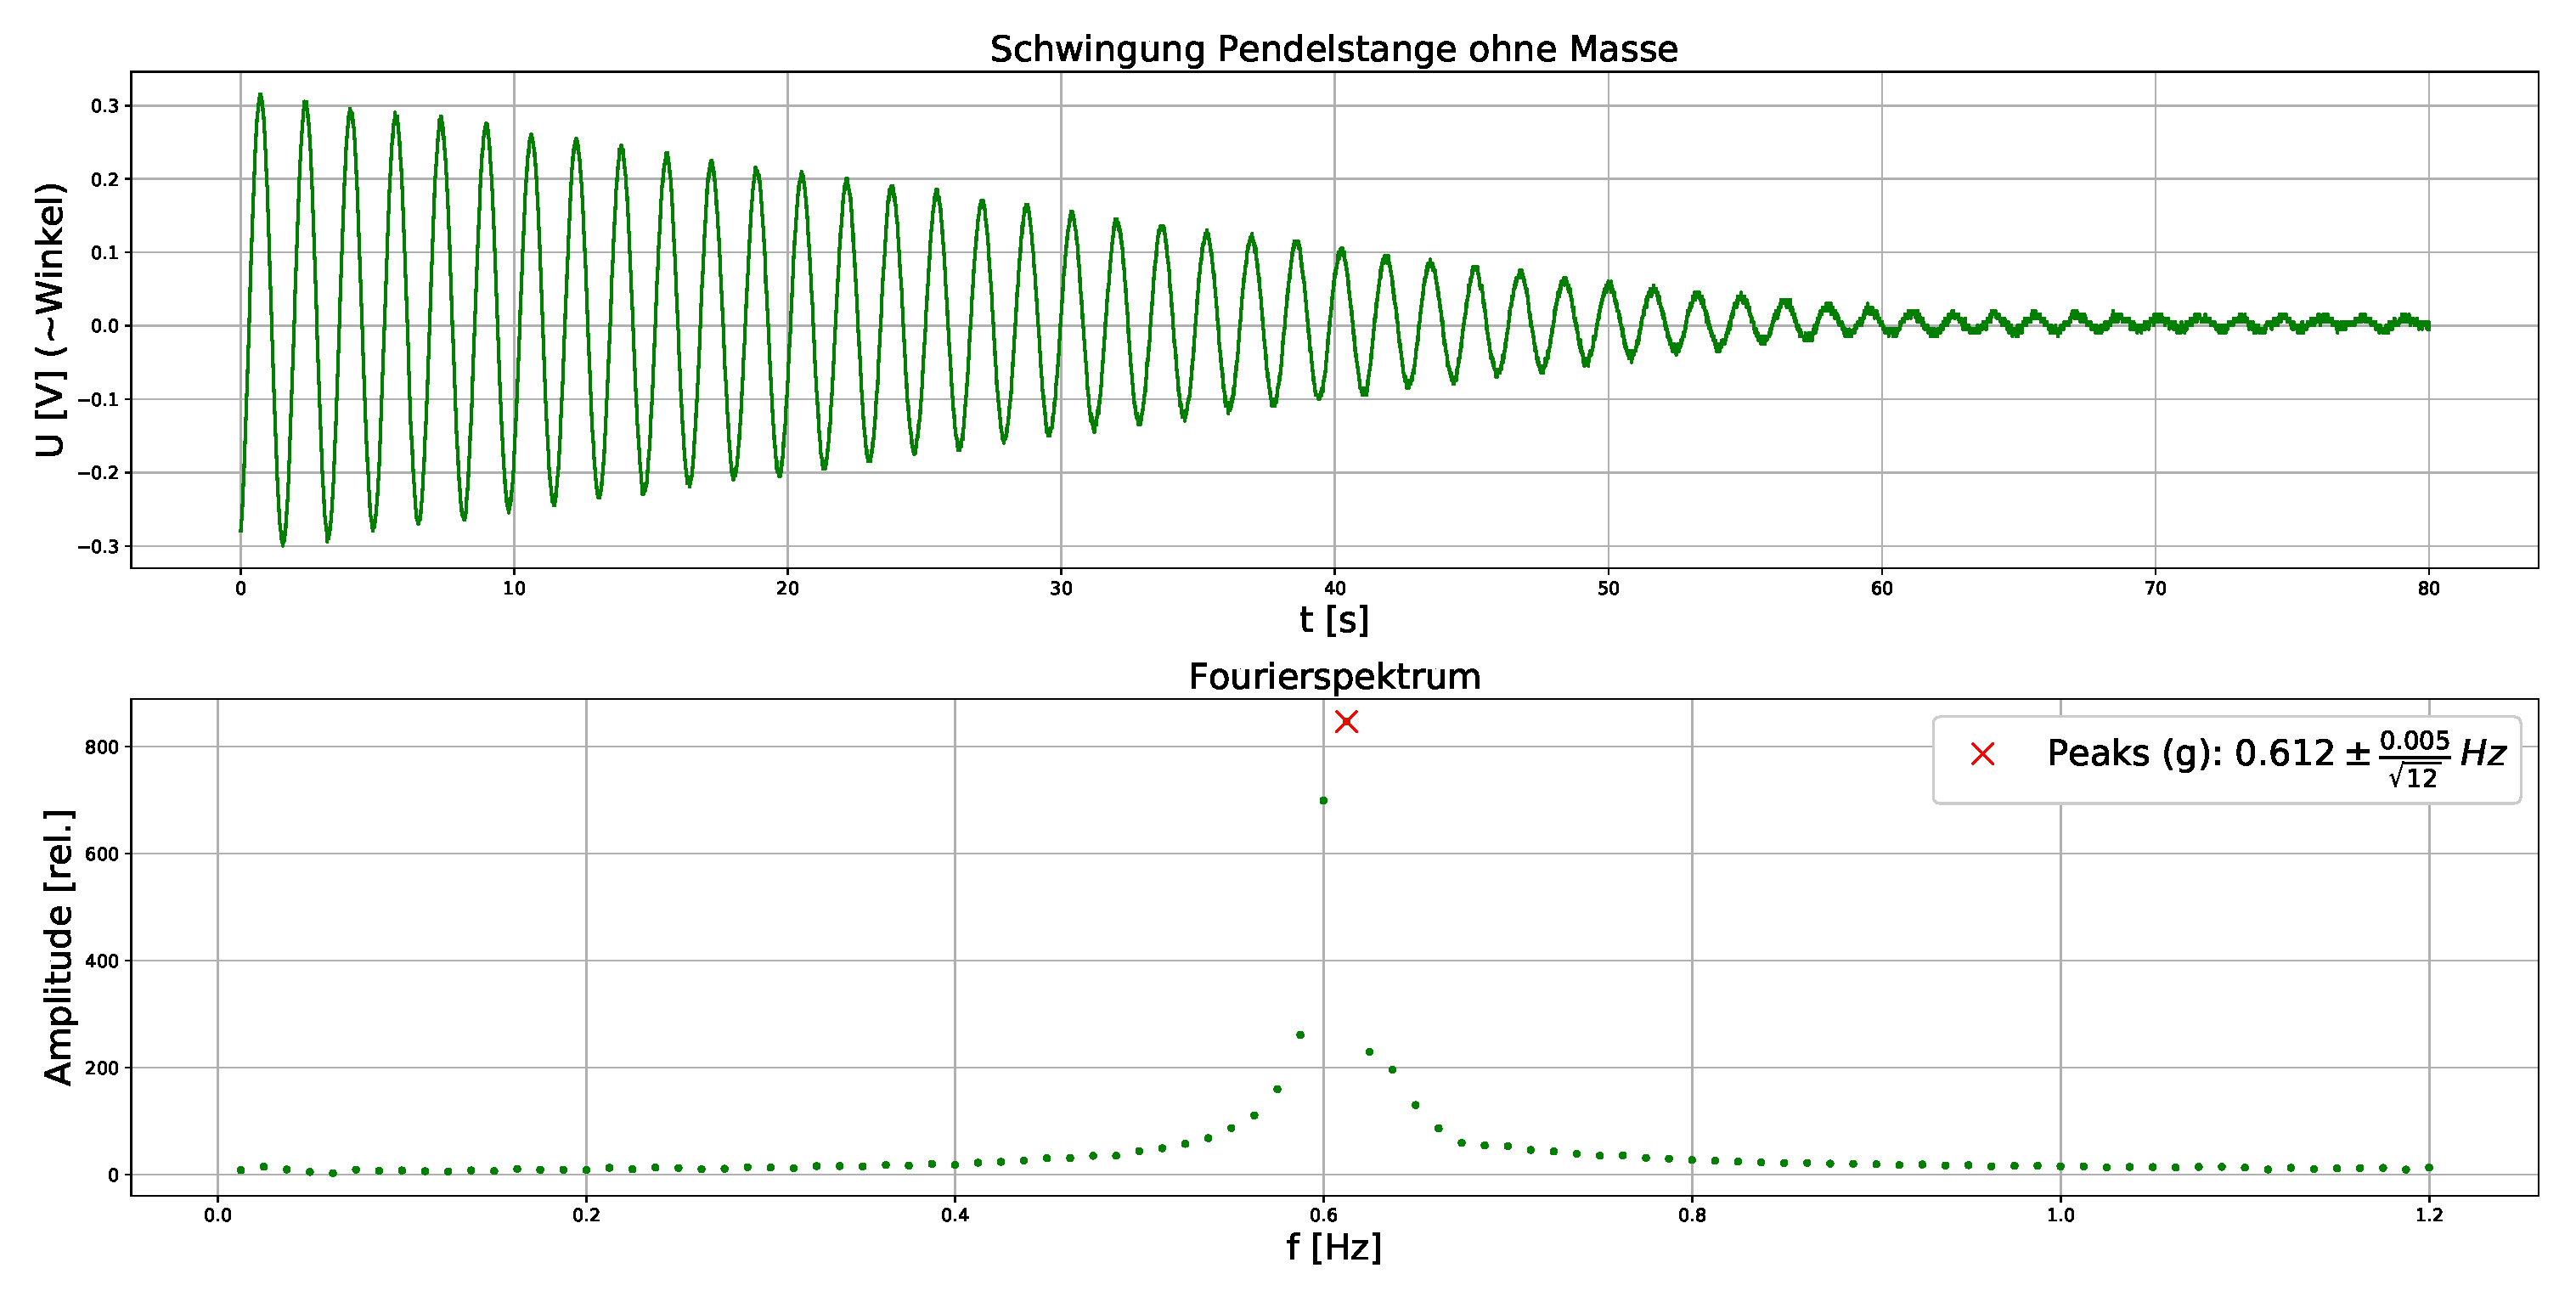
\includegraphics[width=1\textwidth,height=0.75\textheight]{Stange.eps}
\end{figure}
\end{frame}

\begin{frame}{Auswertung - FFT: Schwingung Einfachpendel}
\begin{figure}[h]
\centering
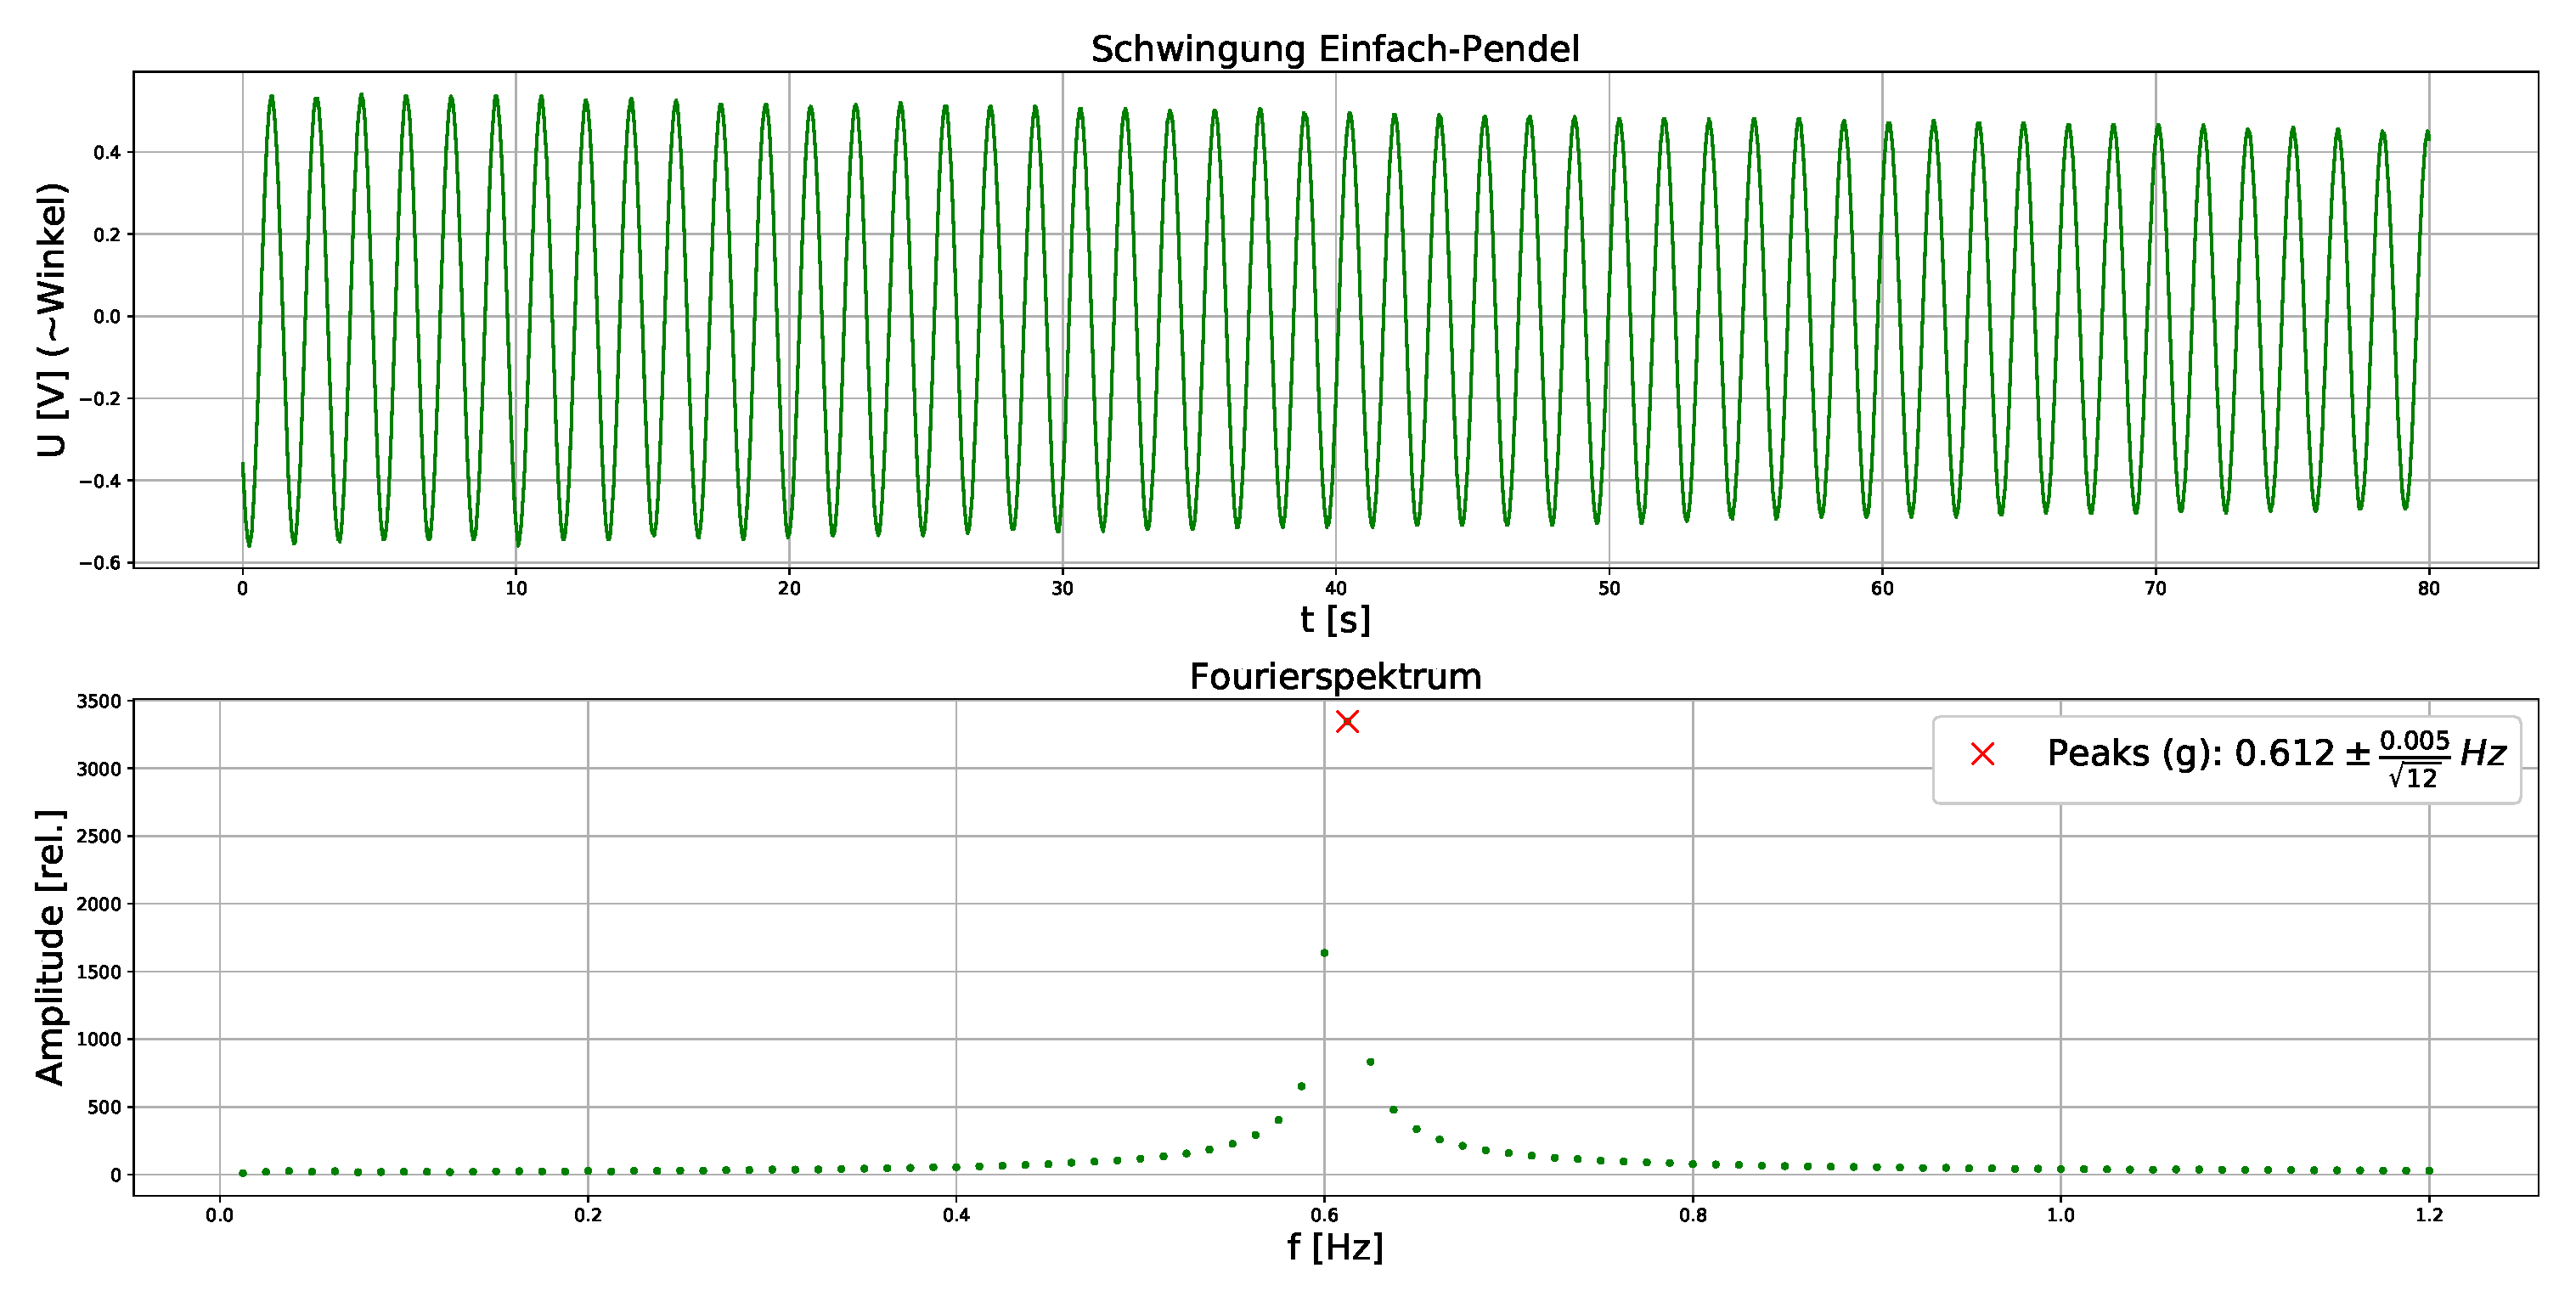
\includegraphics[width=1\textwidth,height=0.75\textheight]{Einfachpendel.eps}
\end{figure}
\end{frame}


\begin{frame}{Auswertung - Messwerte beider Gruppen}

\begin{table}
\small
\centering
\renewcommand{\arraystretch}{1.5}
	\begin{tabular}{ccc}
	\hline
	& Gruppe 1 & Gruppe 2 \\
	\hline
	Frequenz Stange &$0.6061 Hz$ & $0.6075 Hz$ \\
	\hline 
	Frequenz Pendelkörper &$0.6587 Hz$ & $0.6082 Hz$ \\
	\hline
	Kreisfrequenz & $4.0976 \pm 0.0003 Hz$ & $ 3.845 \pm 0.009 Hz$\\
	\hline
	Pendellänge & $ 0.56926 \pm 0.000578 m$ & $0.669 \pm 0.001 m$\\
	\hline
	Erdbeschleunigung & $9.581 \pm 0.0098\frac{m}{s^2} $ & $9.786 \pm 0.049 \frac{m}{s^2}$\\
	\hline
	Abweichung & $\approx 23\, \sigma$ & $0.49\, \sigma$ \\
	\hline
	\end{tabular}
\end{table}

\end{frame}

\begin{frame}{Fazit - Einfachpendel}
\begin{itemize}
	\item Angleichung der Frequenzen von Stange und Pendel hat bei den Gruppen unterschiedlich gut funktioniert
	\item Durch Mehrfachmessung der Länge konnte eine Gruppe den Fehler stark verringern (daher $\sigma$-Abweichung vom wahren Wert umso höher)
	\item Aufgrund von großem Fehler liegt $g$-Wert einer Gruppe innerhalb von einem $\sigma$
\end{itemize}
\end{frame}



\begin{frame}{gekoppeltes Pendel - Grundlagen}
\begin{itemize}
	\item Bewegungsgleichung (analog für zweites Pendel)
	\begin{equation*}
	M_1 = J \cdot \ddot \phi_1 = -m \cdot g \cdot l_S \cdot \phi_1 - D_F \cdot l_F^2 \cdot (\phi_2 - \phi_1)
	\end{equation*}
	\item gleichsinnige Schwingung
	\begin{equation*}
	\phi_i(t) = \phi_{max} \cdot cos(\omega_S t) \; mit \; \omega_S = \frac{mgL_S}{J}
	\end{equation*}
	\item gegensinnige Schwingung
	\begin{equation*}
	\phi_i(t) = (-)\phi_{max} \cdot cos(\omega_{Sf} t) \; mit \; \omega_{Sf}^2 = \omega_S^2 + 2\Omega^2 \; und \; \Omega = \frac{D_F L_F^2}{J}
	\end{equation*}
	\item Schwebung
	\begin{equation*}
	\phi_i(t) = \phi_{max} \cdot \cos(\omega_{sch} t)\cos(\omega_k t) \; mit \; \omega_{k,sch} = \frac{\omega_{Sf} \pm \omega_S}{2}
	\end{equation*}
\end{itemize}
\end{frame}

\begin{frame}{gekoppeltes Pendel - Grundlagen}
\begin{itemize}
	\item der Kopplungsgrad ist definiert als
	\begin{equation*}
	\kappa = \frac{\Omega^2}{\omega_S^2 + \Omega^2} = \frac{D_F L_F^2}{mgL_s + D_F L_F^2 }
	\end{equation*}
	\item daraus erhält man die Federkonstante
	\begin{equation*}
	\Rightarrow \quad D_F = \frac{mgL_s}{\left(\frac{1}{\kappa}-1\right) L_F^2 } 
	\end{equation*}
	
\end{itemize}
\end{frame}



\begin{frame}{gekoppeltes Pendel - Versuchsaufbau}
\begin{figure}
	\centering
	\includegraphics[scale=0.6]{Selection_074.jpg}
\end{figure}
\end{frame}


\begin{frame}{gekoppeltes Pendel - Versuchsdurchführung}
\begin{itemize}
\item Pendel so positionieren, dass Feder in Ruhelage gespannt ist (Pendel daher nicht mehr vertikal) 
\item Fälle:
	\begin{enumerate}
		\item beide Pendel in selbe Richtung auslenken
		\item in entgegengesetzte Richtungen auslenken
		\item ein Pendel auslenken, das Andere in Ruhelage lassen
	\end{enumerate}
\item nicht zu weit auslenken, um Kleinwinkelnäherung zu behalten
\item beachten, dass Pendel stets in einer Ebene ausgelenkt werden
\end{itemize}
\end{frame}

\begin{frame}{Auswertung - gleichsinnige Schwingung}
\begin{figure}[t]
	\centering
	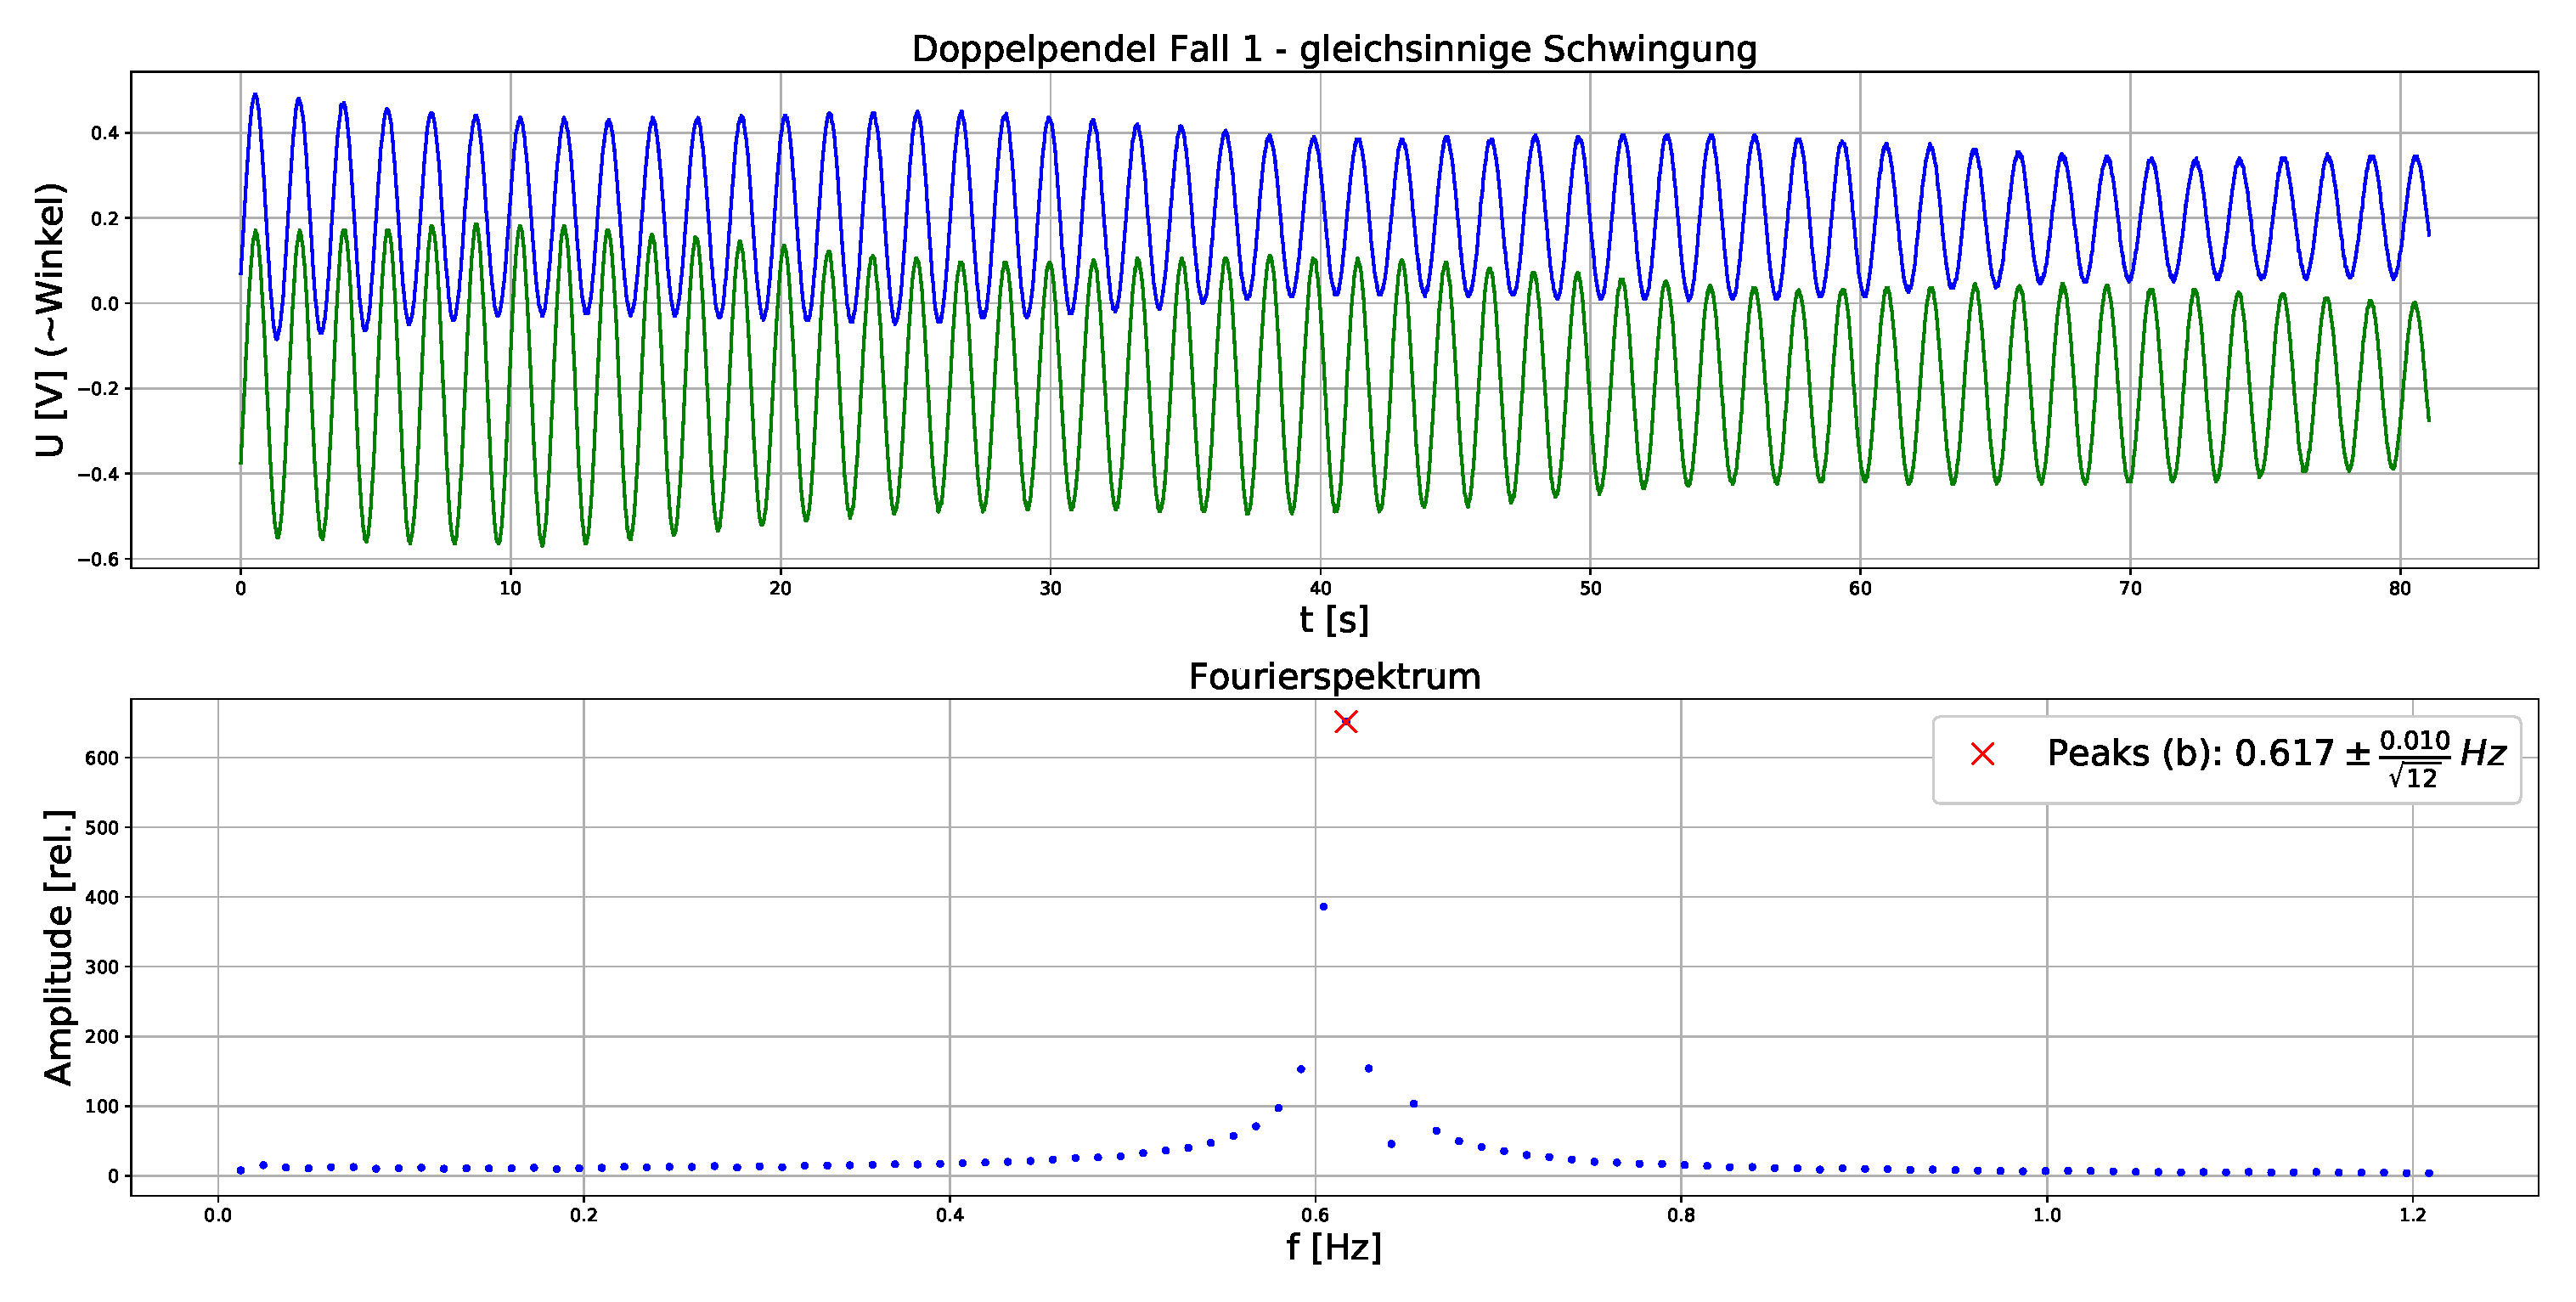
\includegraphics[width=1\textwidth,height=0.7\textheight]{Doppelpendel1.eps}
\end{figure}
\begin{equation*}
\omega_s = 3.877 \pm 0.018 Hz
\end{equation*}
\end{frame}

\begin{frame}{Auswertung - gegensinnige Schwingung}
\begin{figure}[t]
	\centering
	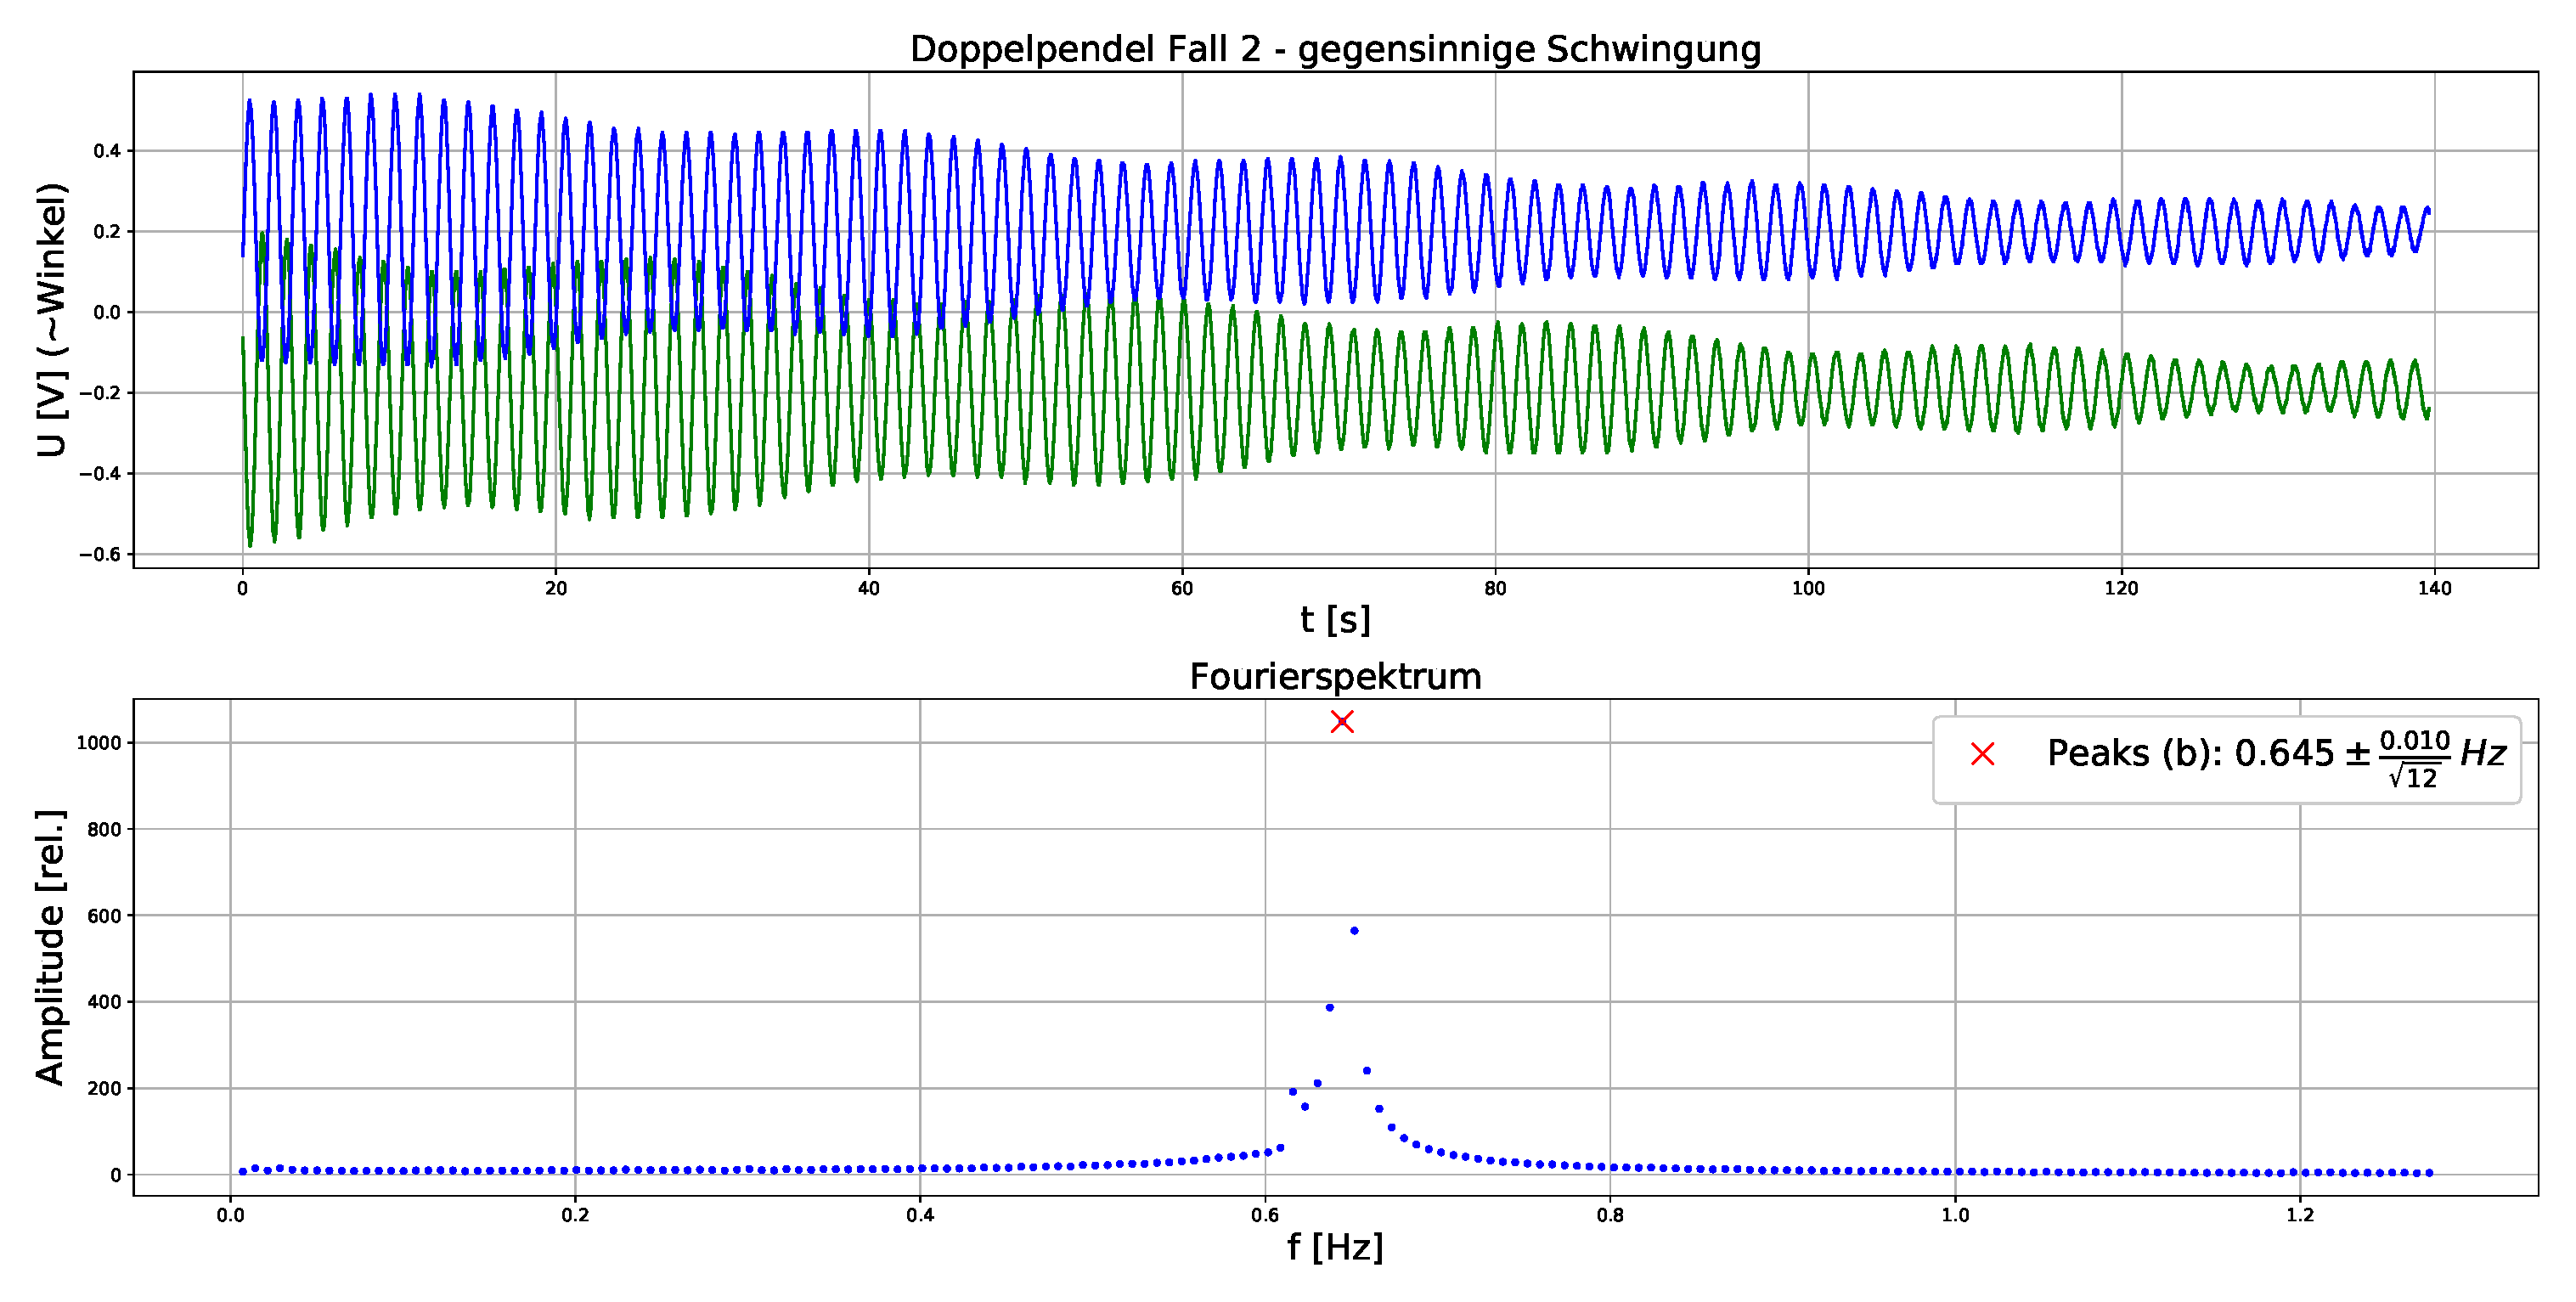
\includegraphics[width=1\textwidth,height=0.7\textheight]{Doppelpendel2.eps}
\end{figure}
\begin{equation*}
\omega_{sf} = 4.053 \pm 0.018 Hz
\end{equation*}
\end{frame}

\begin{frame}{Auswertung - Schwebung}
\begin{figure}[t]
	\centering
	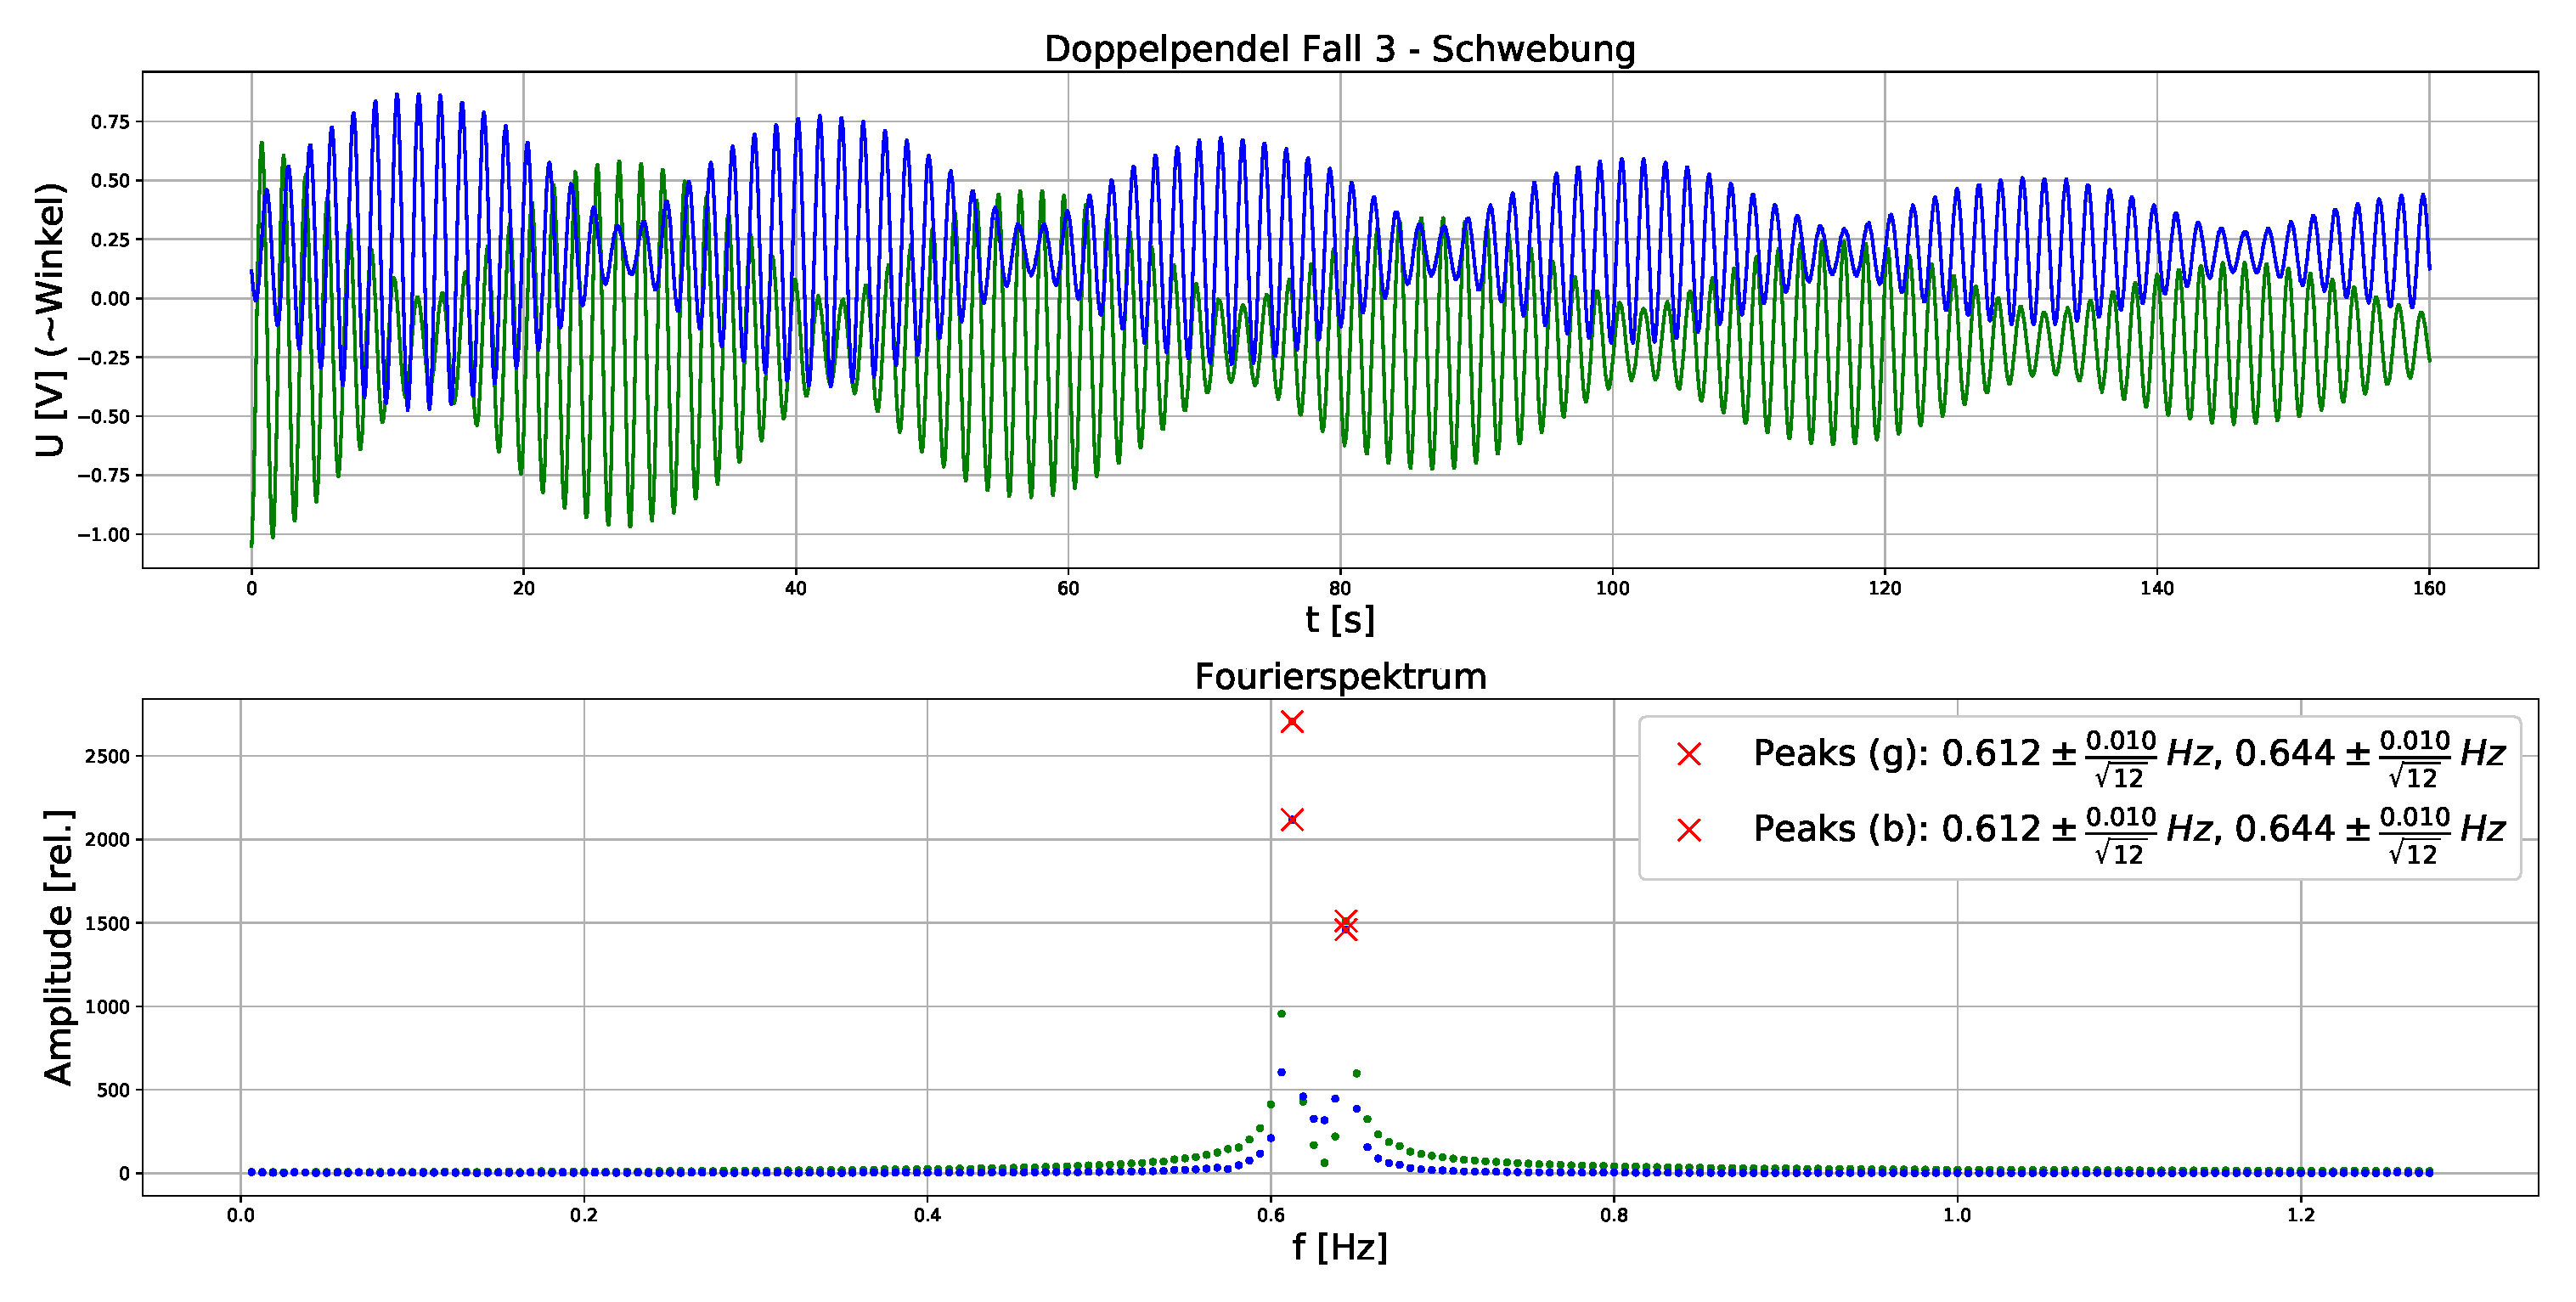
\includegraphics[width=1\textwidth,height=0.7\textheight]{Doppelpendel3.eps}
\end{figure}
\begin{equation*}
\omega_k = 4.046 \pm 0.018 Hz \qquad \omega_{sch} = 3.845 \pm 0.018 Hz
\end{equation*}
\end{frame}

\begin{frame}{Auswertung - Bestimmung der Kopplung}
\begin{itemize}
	\item zunächst Bestimmung der Frequenz $\Omega = \frac{D_Fl_F^2}{J}$:
		\begin{equation*}
		\Omega = \sqrt{\frac{\omega_{sf}^2-\omega_s^2}{2}} = 0.835 \pm 0.009 Hz
		\end{equation*}
	\item damit Bestimmung des Kopplungsgrads:
		\begin{equation*}
			\Rightarrow \kappa = \frac{\Omega^2}{\omega_s^2 + \Omega^2} = 0.0462 \pm 0.0003
		\end{equation*}
	\item mit der Masse $m = 1021.2 \pm \frac{0.1}{\sqrt{12}} g$ und Federposition $L_F = 0.285 \pm 0.001 m$ ergibt sich die Federkonstante:
		\begin{equation*}
			D_F = \frac{mgL_s}{\left(\frac{1}{\kappa}-1\right) L_F^2 } = 3.987 \pm 0.044 \frac{kg}{s^2}
		\end{equation*}
\end{itemize}

\end{frame}

\begin{frame}{Fazit - gekoppeltes Pendel}
\begin{itemize}
\item es war schwierig, die Pendel in einer Ebene auszulenken und die Anfangsbedingungen zu beachten
\item mehr Unterschied zwischen $\omega_k$ und $\omega_{sch}$ erwartet
\item Fehler durch $g$-Messung fließt am stärksten in $D_F$ ein
\item mit Messungen für mehrere Federposition hätte man das $D_F$ durch lineare Regression bestimmen können
\end{itemize}
\end{frame}


\end{document}